\documentclass[]{article}
\usepackage{graphicx}
\usepackage{amsmath}
\usepackage{hyperref}
\usepackage{url}
%opening
\title{Dynamics Derivation for Cart Inverted Pendulum}
\author{Tianpeng Zhang}

\begin{document}

\maketitle

\begin{figure}[!ht]
	\centering
	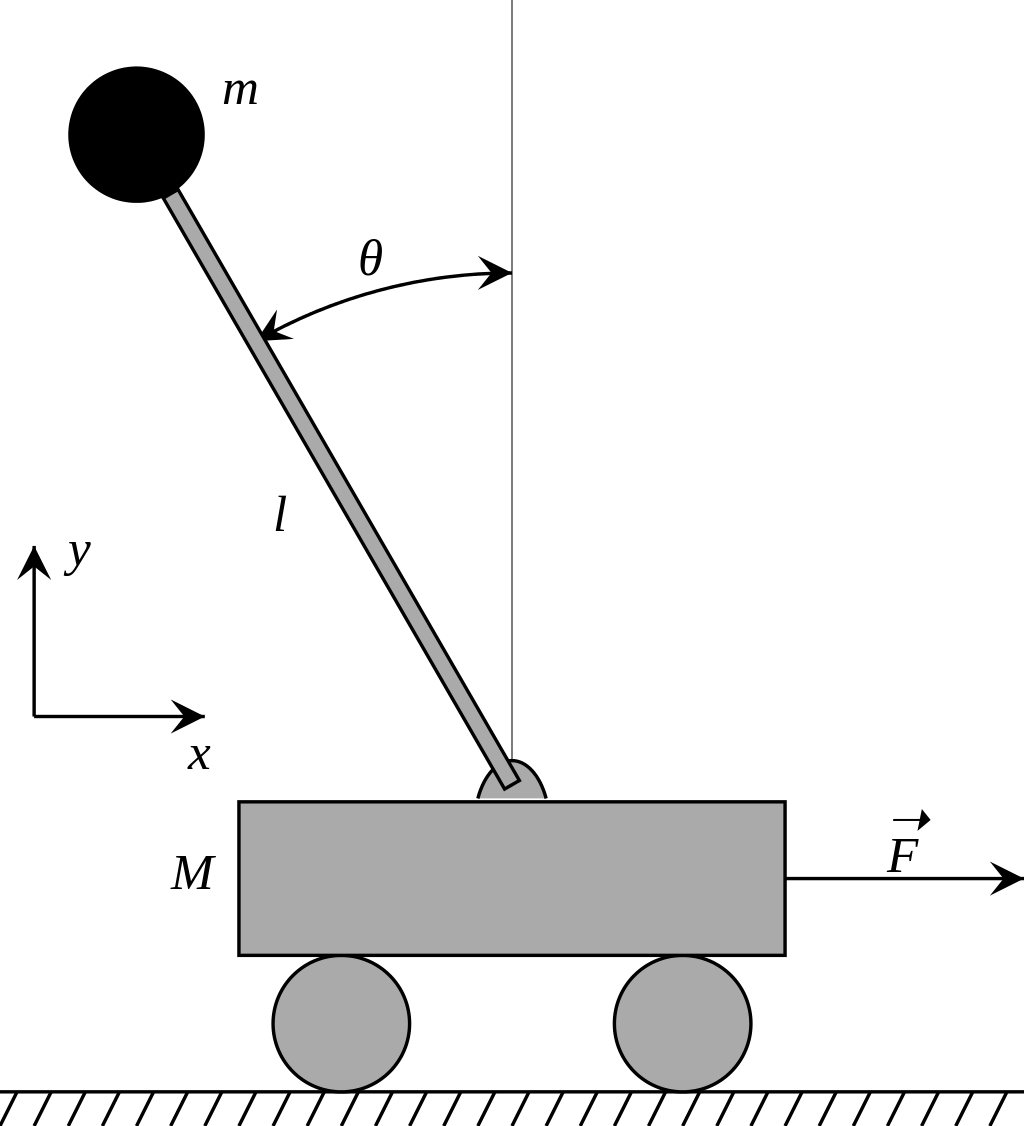
\includegraphics[width=0.5\linewidth]{Cart-pendulum}
	\caption{Forces and Coordinate System for Cart Inverted Pendulum}
	\label{fig:cart-pendulum}
\end{figure}

See Figure \ref{fig:cart-pendulum} for the forces acted on the system. We assume the rod connected the cart $M$ and the weight $m$ is massless, and ignore any drag/friction in the system. The most important external forces are gravity on the weight $m$ and our control input force $F$.


See \href{https://en.wikipedia.org/wiki/Inverted_pendulum#Inverted_pendulum_on_a_cart}{this Wikipedia Page} for the derivation of the following equation of motions:

\begin{equation}\label{eq:of_motion}
	\begin{split}
	&(M+m)\ddot{x} - ml\ddot{\theta}\cos\theta + ml\dot{\theta}^2\sin\theta = F\\
	&l\ddot{\theta}-g\sin\theta = \ddot{x}\cos\theta
	\end{split}
\end{equation}
 

Notice from the second equation in \eqref{eq:of_motion}, 

\begin{equation}\label{eq:xddot}
	\ddot{x} = (l\ddot{\theta}-g\sin\theta )/\cos\theta
\end{equation}

Substitute \eqref{eq:xddot} into the first equation in \eqref{eq:of_motion}, can get $\ddot{\theta}$ as

\begin{equation}\label{eq:thetaddot}
	\ddot{\theta} = [(M+m)g\sin\theta - ml\dot{\theta}^2\sin\theta\cos\theta + F\cos\theta]/(M+m\sin^2\theta)l
\end{equation}

Notice $\ddot{\theta}$ does not depend on $x,\dot{x}$, therefore the $(\theta,\dot{\theta})$ subsystem it can be treated as an isolated system.

And substitute \eqref{eq:thetaddot} into \eqref{eq:xddot} we get $\ddot{x}$ as

\begin{equation}
	\ddot{x} = (mg\sin\theta\cos\theta-ml\dot{\theta}^2\sin\theta + F)/(M+m\sin^2\theta)
\end{equation}

Let's denote the system state vector as $s$, which contains four elements: $s=(x,\dot{x},\theta,\dot{\theta})$. Let us denote $u=F$ as the control input. The state transition function for $s$ is then

\begin{equation}
	\dot{s}=\begin{bmatrix}
	s_2\\
	(mg\sin s_3\cos s_3-ml s_4^2\sin s_3 + u)/(M+m\sin^2 s_3)\\
	s_4\\
	[(M+m)g\sin s_3 - ml s_4^2\sin s_3\cos s_3 + u\cos s_3]/(M+m\sin^2 s_3)l
	\end{bmatrix}
\end{equation}

Again, notice the $(s_3,s_4)$ subsystem can be treated as an isolated system.
\end{document}
